%%%%%%%% ICML 2021 EXAMPLE LATEX SUBMISSION FILE %%%%%%%%%%%%%%%%%

\documentclass{article}

% Recommended, but optional, packages for figures and better typesetting:
\usepackage{microtype}
\usepackage{graphicx}
\usepackage{subfigure}
\usepackage{booktabs} % for professional tables
\usepackage{multirow}
% hyperref makes hyperlinks in the resulting PDF.
% If your build breaks (sometimes temporarily if a hyperlink spans a page)
% please comment out the following usepackage line and replace
% \usepackage{icml2021} with \usepackage[nohyperref]{icml2021} above.
\usepackage{hyperref}

% Attempt to make hyperref and algorithmic work together better:
\newcommand{\theHalgorithm}{\arabic{algorithm}}


\usepackage[accepted]{icml2021}

\icmltitlerunning{Wine Quality Prediction}

\begin{document}

\twocolumn[
\icmltitle{Wine Quality Prediction}

\begin{icmlauthorlist}
\icmlauthor{Stijn de Preter (852726504)}{ou}
\icmlauthor{Arjan Broer (850166428)}{ou}
\end{icmlauthorlist}

\icmlaffiliation{ou}{Open Universiteit}
\icmlcorrespondingauthor{}{}

% You may provide any keywords that you
% find helpful for describing your paper; these are used to populate
% the "keywords" metadata in the PDF but will not be shown in the document
\icmlkeywords{wine quality, machine learning, neural networks, ANN, SVR }

\vskip 0.3in
]

\section{Brief Introduction}
The assignment is based on the article \cite{dahal2021prediction} and focuses on the reproduction of the article results.
The reproduct is limited to only the Support Vector Regression (SVR) and Artificial Neural Network (ANN) models.
The Ridge Regression (RR) and Gradient Boosting Regression models are not included in this report.
The goal of the assignment is to predict the quality of wine based on its chemical properties and understand the methods used to generate the predictions.
The dataset will be analyzed to find the features that most influence the quality of wine and suggestions are provided to improve the hyperparameters of the model for best results.

The research questions discussed in this report are:
\begin{enumerate}
    \item Reproduce the results of the article \cite{dahal2021prediction} using the same dataset and models.
    \item Analyze the dataset to find the features that most influence the quality of wine.
    \item Provide suggestions to improve the hyperparameters of the model for best results.
\end{enumerate}

\section{Methods}
Describe the methods used. How it works. It can include algorithms, system descriptions, new language constructs, analyses, etc.
Provide diagrams to help in the discussion. Figure \ref{fig:one-col-figure} and Figure \ref{fig:two-col-figure} shows an example of a one-column figure and a two-column figure. 
\begin{figure}
    \centering
    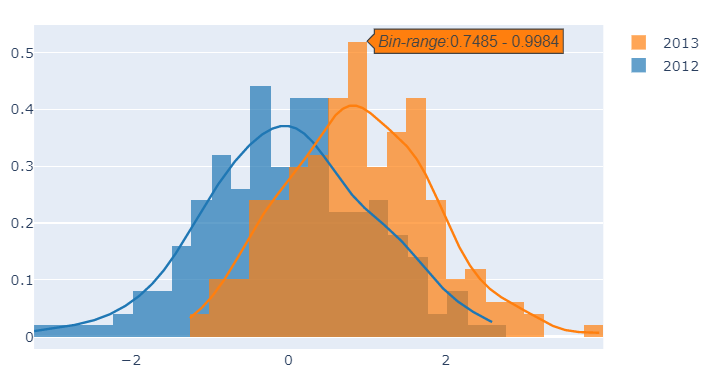
\includegraphics[width=\linewidth]{figures/example_plot.png}
    \caption{One-column figure that explains the steps or framework of your method / model.}
    \label{fig:one-col-figure}
\end{figure}

\subsection{SVR and ANN - Reproduce the results}
In order to compare the results of the article with our results, a visualization was made. Here the values of the article (\textbf{still to be added}) are compared with our results repeatedly. Our results are reproduced repeatedly with different test and training data each time. This way we are sure that it is not a lucky shot but we get a realistic picture of how our model performs.

\subsection{SVR and ANN - Impact of the features}
TBC

\subsection{SVR and ANN - Inprove the model}
TBC

\begin{figure*}
    \centering
    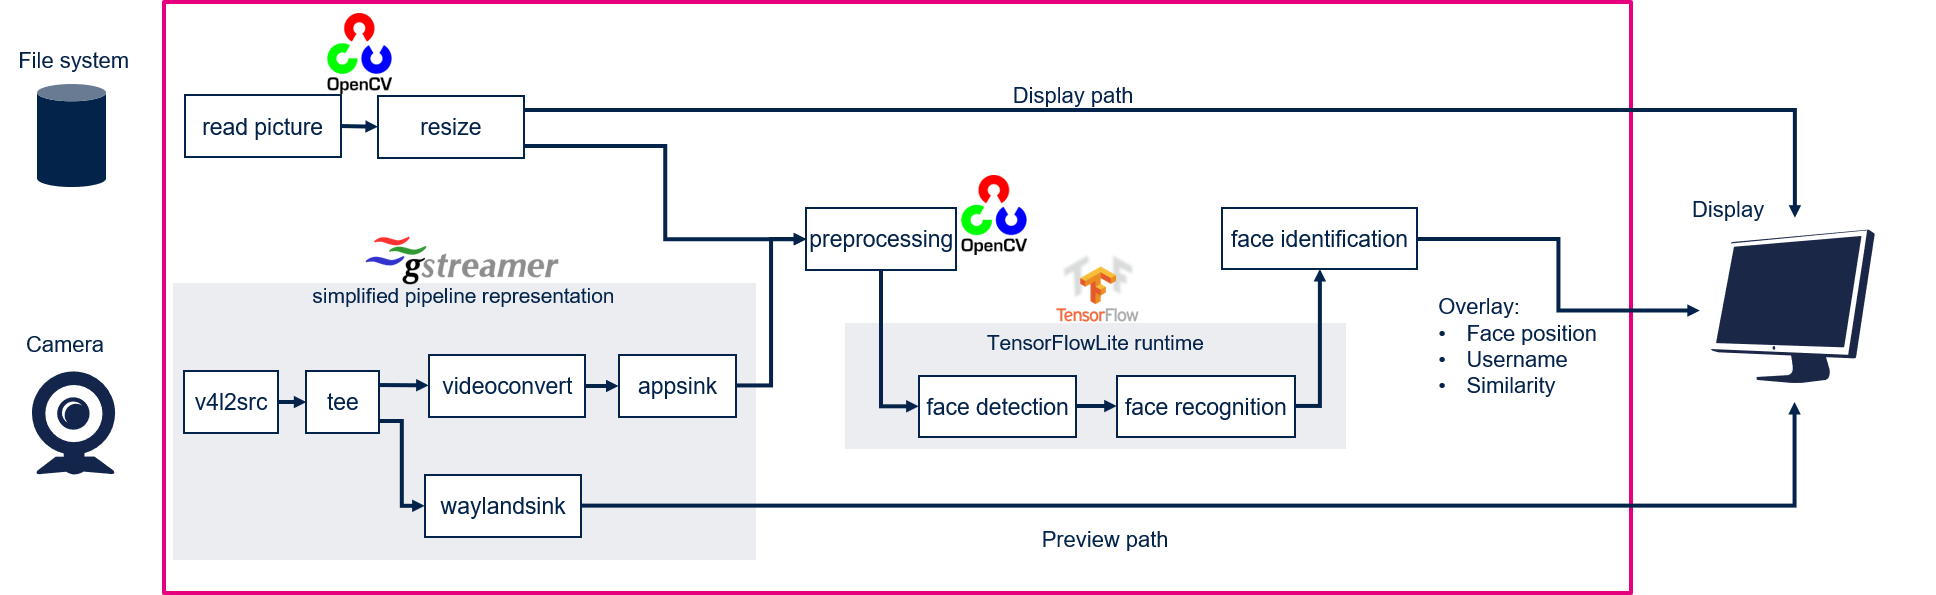
\includegraphics[width=\linewidth]{figures/example_pipeline.png}
    \caption{One-column figure that explains the steps or framework of your method / model.}
    \label{fig:two-col-figure}
\end{figure*}

\section{Experimental Results}

\subsection{SVR}

\subsubsection{Datasets}
Include a description of the data used, what it contains, train test splits, etc.

\textbf{Hier de bevinding schrijven dat het over de white wine ipv de red wine gaat.}

\subsubsection{Implementation Details}
Include a description of the design choices, hyperparameters, and other implementation specific details.





\subsubsection{Results}
Analyze and discuss your results. Table \ref{tab:example-table} shows an example of a table.
Include plots and visualizations such as Figure \ref{fig:one-col-figure}.

\subsubsection{Discussion}
Additionally, you can include a separate discussion section in which you summarize the results, indicate possible limitations of your work, and provide suggestions for future research.

\subsubsection{Citing references}
LaTeX manages the citations for you. You simply have to add the bibtex entry for the reference in the references.bib file and you can use the citation in the paper \cite{langley00}. You can also cite multiple references in one command \cite{DudaHart2nd,Newell81,kearns89}. The bibtex entries for a paper can be obtained in websites such as google scholar or dblp.

\subsection{SVR}

\subsubsection{Datasets}


\subsubsection{Implementation Details}



\subsubsection{Results}


\subsubsection{Discussion}


\subsubsection{Citing references}


\bibliography{references}
\bibliographystyle{icml2021}


\end{document}

